\section{Datenübertragung}
\label{sec:Daten}
Im folgenden wird ein Konzept beschrieben, um Daten des VARAN-Buses optisch und bidirektional zu übertragen. Ausserdem wird eine Sende- und Empfängerschaltung entworfen, um einen Teilbereich des Konzepts zu überprüfen und wichtige Erkenntnisse für die Fortsetzung der Arbeit zu sammeln.  
\subsection{Konzept}
In Abbildung \ref{fig:Konzept_Daten} wird grob das Konzept zur optischen Datenübertragung gezeigt.

\begin{figure}[h]
	\centering
	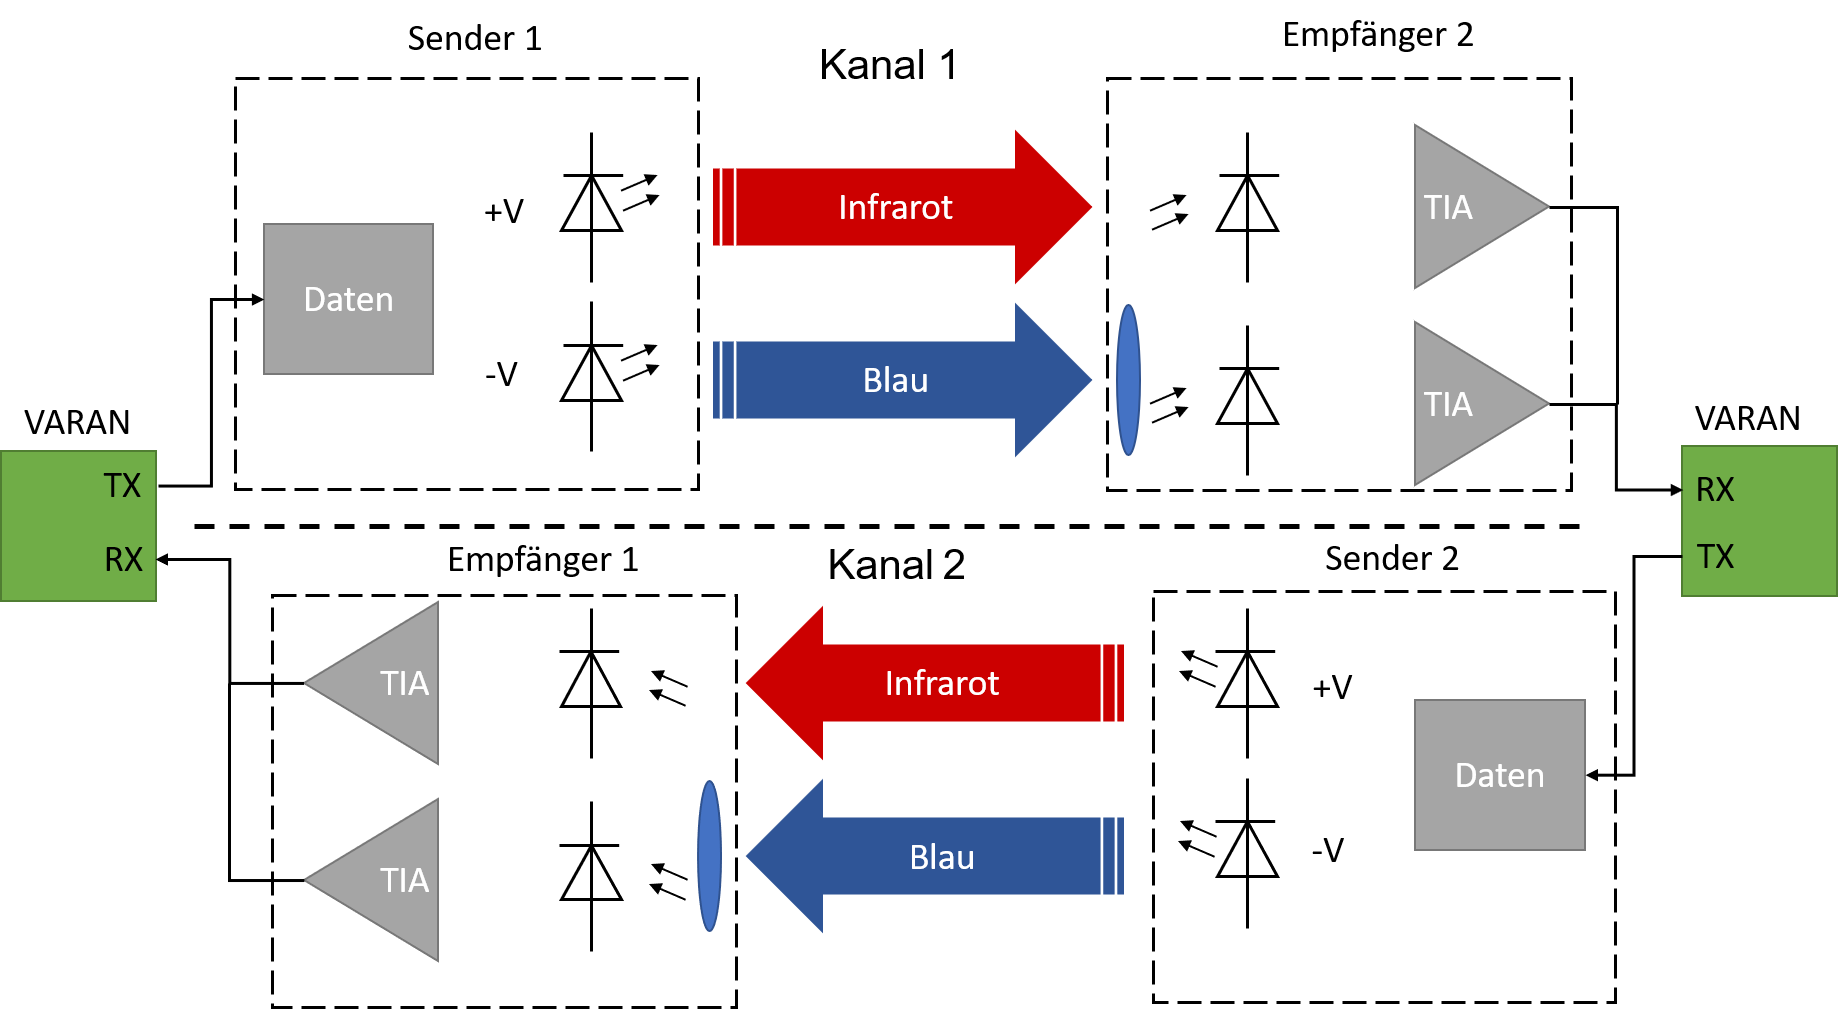
\includegraphics[width=\linewidth]{Konzept_Daten.png}
	\caption{Konzept der optischen Datenübertragung}\label{fig:Konzept_Daten}
\end{figure}

In der Abbildung sind die beiden Kanäle zu erkennen, welche optisch voneinander getrennt sind. Jeder Kanal überträgt dabei die Daten nur in jeweils eine Richtung. Beide Kanäle zusammen sorgen für die gewünschte Bidirektionalität. Auf der Primär- und Sekundärseite hat es jeweils eine Sende- und Empfangseinheit. Eine Sendeeinheit besteht aus der Datenerfassung und den Leuchtdioden. Da der VARAN-Bus MLT-3 codiert ist, müssen drei Zustände übertragen werden können. Die positiven Spannungspegel werden mit einer Infrarot-LED übertragen und die negativen Spannungspegel mit einer blauen LED. Der Zustand \glqq0\grqq steht an, wenn keine der LEDs leuchtet.
\newline
Eine Empfangseinheit besteht aus Photodioden und Verstärkerschaltungen. Im blauen Spektralbereich werden mit Hilfe eines optischen Filters vor der Photodiode die unerwünschten Spektralanteile herausgefiltert.
\newline Die beiden Sende- und Empfangseinheiten sind identisch aufgebaut und unterscheiden sich nur in der Übertragungsrichtung.

\paragraph{Sender}
In folgender Abbildung wird das Konzept einer Sendeeinheit detaillierter beschrieben.
\begin{figure}[h]
	\centering
	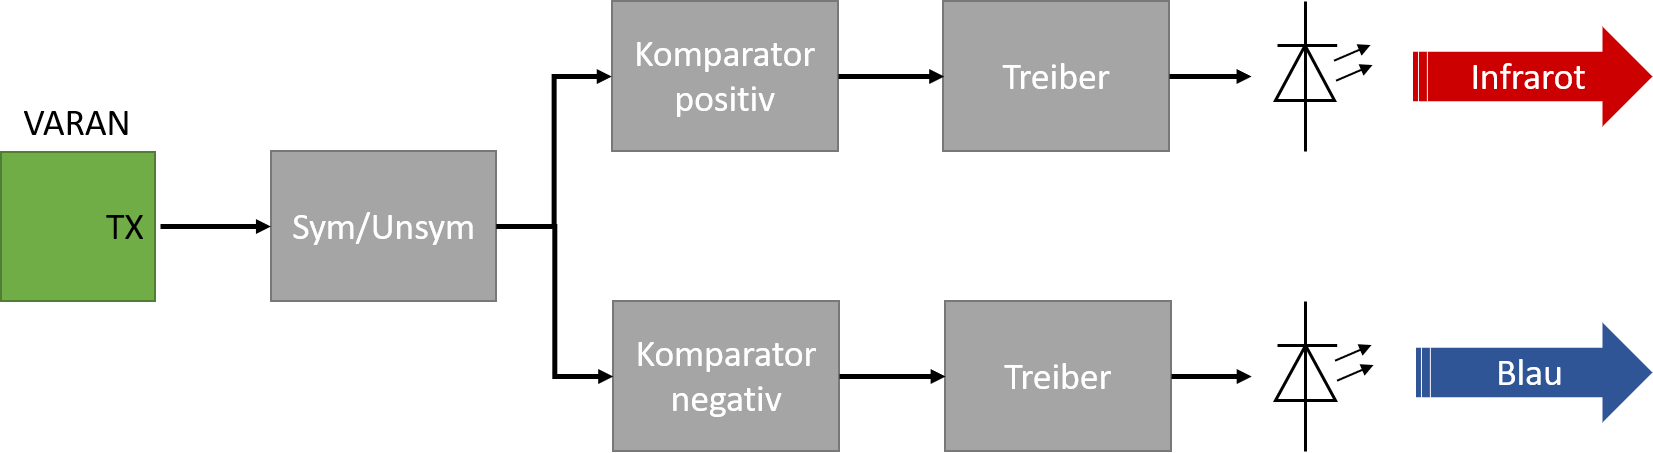
\includegraphics[width=\linewidth]{Konzept_Sender.png}
	\caption{Konzept der optischen Sendeeinheit}\label{fig:Konzept_Sender}
\end{figure}
\paragraph{Empfänger}
In folgender Abbildung wird das Konzept einer Empfangseinheit detaillierter beschrieben.
\subsection{Dimensionierung}
Hier wird auf die Dimensionierung der Schaltung eingegangen.
\subsection{Simulation}
Im Simulations-Abschnitt wird die Dimensionierung und das Konzept überprüft.
\subsection{Testaufbau}
In diesem Unterkapitel wird der Testaufbau beschrieben.